\documentclass[letterpaper]{article}
\linespread{2}
\usepackage{fullpage}
\usepackage{ngerman}
\usepackage{graphicx}


\begin{document}

	\title {Studienarbeit\\Modelle verteilter Systeme}
	\author {Prof. Dr. Ralph Lano\\ \\ \\Jasmin H. Paszko - Medieninformatik\\XXXXXXXX} %put your name and student ID here
	\date {Fall 2008}
	\maketitle

\newpage
	\tableofcontents
	
\newpage
	
\section{Projekt Autorennspiel}
Gruppe 2\\
(urspr\"unglich GER-Gruppe 5, US-Gruppe 2)
\subsection{Projektbeschreibung}
Als Projekt wurde im Vorfeld ein 3D-Autorennspiel auf der XBOX-360 Plattform festgelegt.\\
Die Mitglieder des Teams sind:
\begin{itemize}
	\item Claus Wollnik (ger)
	\item Mike Kotsch (ger)
	\item Johann Vogl (ger)
	\item Denis Sinner (ger)
	\item Maximilian F�rster (ger)
	\item Tobias Feigel (ger)
	\item Chris Kearse (us)
	\item Jasmin Paszko (ger)
	\item Shane Moore (us)
	\item Ron Malcom (us)
\end{itemize}
Vorgabe unserer amerikanischen Kollegen war ein Autorennspiel, das als Rennstrecke den Campus des Abington-Colleges vorgesehen hat. Nach unserem Beitritt zum Team kam die Idee auf, auch den Campus der Hochschule Hof mit in das Spiel zu integrieren, welcher aus Zeitgr\"unden auch der einzige Track geblieben ist.\\
\\
Das Spiel selbst sollte sowohl von einem Einzelspieler als auch von zwei Spielern via Splitscreen oder Netzwerkverbindung gespielt werden k\"onnen. Dahingehende Architekturentscheidungen sind bereits ins Projekt eingeflossen, aber die Umsetzung der Mehrspielermodi und mehrerer w\"ahlbarer Spielerautos konnte nicht mehr eingebaut werden. Nach dem Start des Spiels soll der Spieler im Hauptmen\"u die Optionen und Credits angezeigt bekommen. W\"ahrend des ganzen Spiels soll Sound im Hintergrund h\"orbar sein. 


\subsection{Anforderungen \& Spezifikationen}
Die grunds\"atzliche Anforderung an das Spiel war, dass es sich um ein Autorennspiel in einer 3D-Umgebung handeln sollte. Als Plattform f\"ur das Spiel waren die XBOX-360 und der PC vorgesehen. Als Fahrzeuge sollen Golf-Carts zur Verf\"ugung stehen, die im Spielmen\"u ausgew\"ahlt werden k\"onnen.\\
\\
Das Fahrzeug selbst wird aus der Vogelperspektive gesteuert. Die Geschwindigkeit und eine verkleinerte Kartenansicht sollten an den R\"andern des Bildschirms angezeigt werden. Ebenso soll eine grundlegende Physik geschaffen werden, die Beschleunigung, Abbremsen und Lenken und urspr\"unglich auch Kollisionen mit dem Fahrbahnrand ber\"ucksichtigt.\\
\\
Als 3D-Modelle sollten die Golf-Carts, verschiedene B\"aume, Gras, umliegendes Terrain sowie parkende Autos erstellt werden. Ebenso sollten Geb\"aude in die Karte integriert werden.
Als HUD-Elemente wurden 2D-Assets verwendet, welche die Tachonadel samt Anzeigeblatt und die Mini-Map darstellen. \\
\\
Um die Umsetzung des Projektes zu planen wurde ein Zeitplan erstellt.\\


\begin{center}
	\begin{figure}
		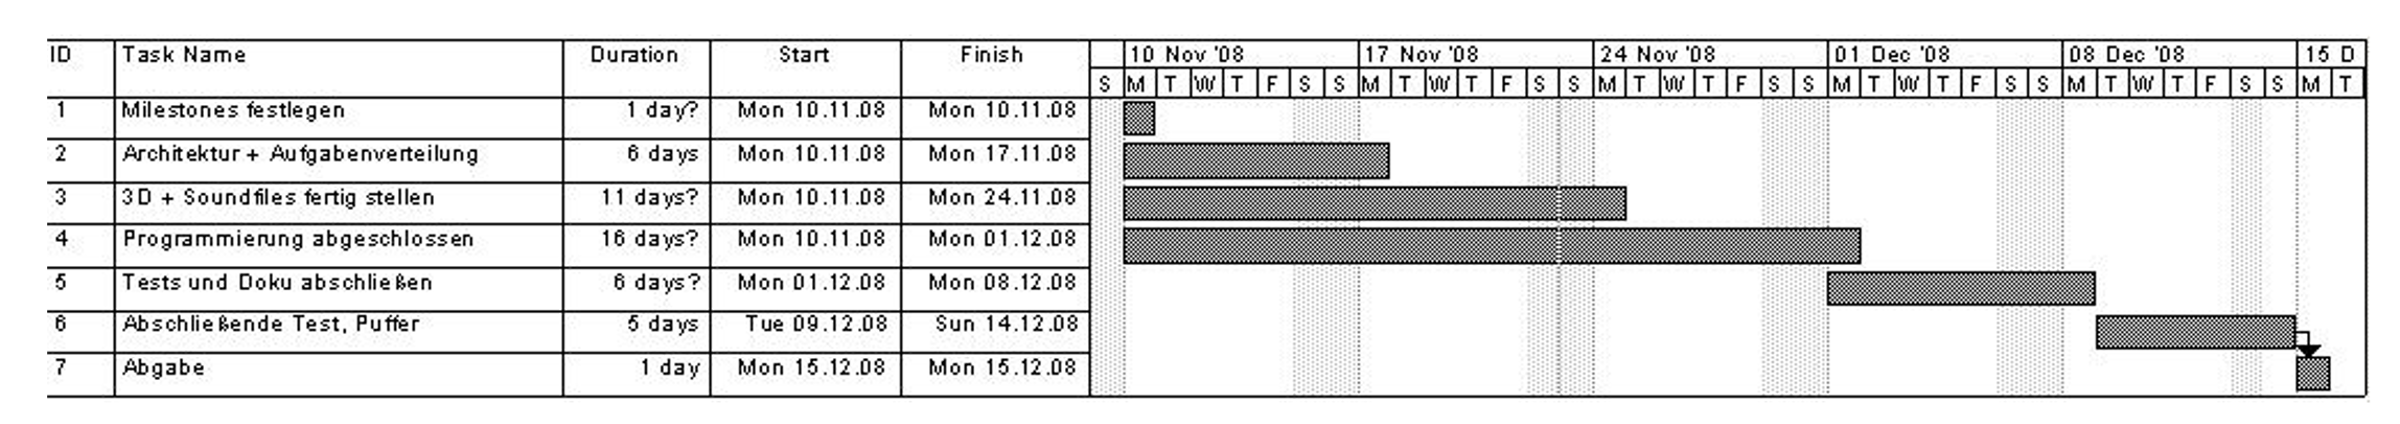
\includegraphics[height=3cm]{milestones.png}
		\caption{Zeitplan und Meilensteine des Projektes}
	\end{figure}
\end{center}


\subsection{Aufgabenverteilung}
Innerhalb der Gruppe gab es verschiedenen Themen zu behandeln. Diese Aufgaben wurden wie folgt verteilt:
\begin{tabbing}
xxxxxxxxxxxxxxxxxxxxx						\=	xxxxxxxxxxxxxxxxxx\kill
Projektleitung:	\>Ron Malcom und Claus Wollnik\\
3D-Objekte:			\>Shane Moore, Denis Sinner, Maximilian F\"orster\\
HUD:						\>Chris Kearse \\
Cardesign:			\>Shane Moore\\
Trackdesign:		\>Mike Kotsch und Johann Vogl\\
Physikengine:		\>Tobias Feigel\\
Sound / Musik:	\>Jasmin Paszko\\
Kamera:					\>Denis Sinner,  Shane Moore\\
Grafikengine:		\>Denis Sinner\\
Programmierung:	\>Jasmin Paszko, Maximilian F\"orster, Denis Sinner, Tobias Feigel, Claus Wollnik\\
								\>und Ron Malcom\\
Dokumentation:	\>Maximilian F\"orster\\
\end{tabbing}

\subsection{Design - UML-Diagramme}
Das folgende Use Case-Diagramm zeigt die verschiedenen M\"oglichkeiten auf, zwischen denen der Benutzer des Autorennspiels w\"ahlen kann.

\begin{center}
	\begin{figure}
	\hspace{5.5cm}
		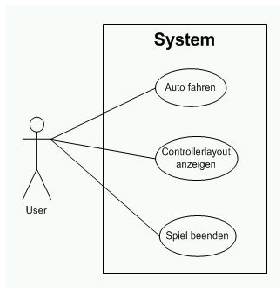
\includegraphics[width=4cm]{usecase.png}
		\caption{Use Case-Diagramm}
	\end{figure}
\end{center}


Abbildung 3 zeigt das Klassendiagramm welches die Beziehungen und das Zusammenspiel der einzelnen Klassen des Projektes verdeutlicht.


\begin{center}
	\begin{figure}
		\hspace{4.5cm}
		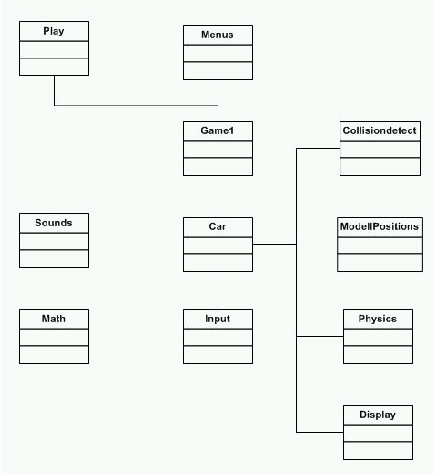
\includegraphics[width=7cm]{classes.png}
		\caption{Klassendiagramm}
	\end{figure}
\end{center}

\subsection{Tools}
Einige Tools wurden als Standard innerhalb der Gruppe vereinbart.
Google-Group wurde als eine Art Forum und Mailingliste festgelegt. Hier k\"onnen alle Themen besprochen werden und jeder bekommt Nachrichten in Echtzeit zugestellt. Ebenso k\"onnen innerhalb des Forums Dateien hochgeladen werden, die dann f\"ur alle Gruppenmitglieder zug\"anglich sind. Zus\"atzlich wurden ebenfalls die E-Mail-Adressen der Teammitglieder untereinander ausgetauscht, um auch direkten Kontakt zu erm\"oglichen. Als Chatprogramm wurde Skype gew\"ahlt, da es neben dem normalen Nachrichtenaustausch auch die M\"oglichkeit der Telefonkonferenz und des Video-Chats erm\"oglicht.\\
\\
F\"ur das Projektmanagement wurde die Website http://act2009.basecamphq.com/clients (Basecamphq) verwendet. Die graphische Darstellung von Zeitplan und Meilensteinen wurde mittels Microsoft Project 2007 erstellt.\\
\\
F\"ur die 3D-Modellierung wurden die Programme Cinema 4D sowie Blender benutzt. Cinema 4D wurde haupts\"achlich aufgrund seiner Plattformunabh\"angigkeit und seiner vielen Zusatzmodule ausgew\"ahlt. F\"ur Blender wurde sich wegen seiner kostenfreien Verf\"ugbarkeit entschieden.\\
\\
Die Texturen wurden haupts\"achlich in Cinema4D erstellt und bearbeitet. Hier hatten die Studenten der Medieninformatik bereits im Vorfeld etliche Erfahrungen gesammelt, und somit war die Wahl dieses Programms nahe liegend.\\
\\
F\"ur die Entwicklung und Programmierung wurde mit Microsoft Visual Studio 2008 und Microsoft XNA-Studio 3.0 die Standard-Software f\"ur Spielentwicklung auf der XBOX-360 gew\"ahlt. Mit diesen Programmen konnte eine h\"ochstm\"ogliche Kompatibilit\"at gew\"ahrleistet werden. 


\subsection{Risikoanalyse und Vorgehen}
\begin {itemize}
	\item Schwieriges Problem, schwieriger Fehler (\textgreater50\%)
	\begin{enumerate}
		\item XNA-Buch lesen
		\item im Netz recherchieren
		\item andere Mitglieder fragen
		\item Teamleiter informieren, der die Architektur \"uberpr\"uft und gegebenenfalls korrigiert
		\item Teamleiter und Mitglied fragen Professor
		\item Feature wegfallen lassen
	\end{enumerate}
	\item Ausfall eines Mitglieds (\textless30\%)
	\begin{enumerate}
		\item Umverlagerung der Arbeit
		\item Abspecken der bearbeiteten Aufgaben
		\item Wegfall der bearbeiteten Features des Mitglieds
	\end{enumerate}
	\item Arbeitsverweigerung (\textless30\%)
	\begin {enumerate}
		\item mit dem Mitglied Kontakt aufnehmen und Problem ergr\"unden
		\item Problem in der Gruppe diskutieren
		\item Professor als Vermittler einschalten
		\item Mitglied aus Gruppe ausschlie\"sen
	\end {enumerate}
	\item Ausfall E-Mail-Account eines Mitglieds (m\"oglich)
	\begin{enumerate}
		\item Account bei anderem Anbieter erstellen
		\item Zugangsdaten anpassen
	\end{enumerate}
	\item Ausfall Googlegroup (\textless10\%)
	\begin{enumerate}
		\item andere Mailingliste verwenden (z.B. Mikkysoft)
		\item Mailadressliste erstellen und aktuell halten
	\end{enumerate}
	\item Ausfall Googlecode (\textless10\%)
	\begin{enumerate}
		\item SVN-Benutzerdaten werden auf anderen Server verlagert (z.B. Claus Wollnik's Server) und die Verwaltung und Download erfolgt dann von dort
		\item Repository muss regelm\"a\ss{}ig abgerufen werden, um den Datenverlust zu Minimieren
	\end{enumerate}
	\item Ausfall Skype / IRC (\textless10\%)
	\begin{enumerate}
		\item Besprechungsergebnisse in der Googlegroup / der Maillingliste publizieren
	\end{enumerate}
\end{itemize}

\subsection{Literatur \& Weblinks}
\subsubsection{Literatur}
\begin{itemize}
	\item Professional XNA Programming: Building Games for Xbox 360 and Windows with XNA Game Studio 2.0, Benjamin Nitschke
	\item Mathematische Formelsammlung, Lothar Papula
	\item Taschenbuch der Physik, Horst Kuchling
	\item Physik f\"ur Ingenieure, Hering \& Martin \& Stohrer
\end{itemize}

\subsubsection{Weblinks}
\begin{itemize}
	\item http://internetducttape.com/2007/03/03/howto\_google\_code\_hosting\_subversion\_tortoisesvn/
	\item http://msdn.microsoft.com/en-us/library/bb203879.aspx
	\item http://msdn.microsoft.com/en-us/library/bb195053.aspx
	\item http://www.phstudios.com/?q=node/16
	\item http://exdream.no-ip.info/blog/\#XnaRacingGame
	\item http://geekswithblogs.net/bitburner/archive/2008/06/22/123061.aspx
	\item http://creators.xna.com/en-US/education/gettingstarted
	\item http://www.3dtotal.com/ffa/tutorials/tutorialsmax.asp
	\item http://msdn.microsoft.com/en-us/library/bb197293.aspx\#ID2ESBAC
\end{itemize}

\section{Eigenanteil\&Fazit}
% put your own part here
% \\ makes a new line 
\end{document}